\chapter{Examples} \label{ch:examples}
This chapter provides some example applications for running JEGA.
This is not meant to show off the capabilities of JEGA but instead
demonstrate how to use it.  Therefore, all examples in this chapter
will solve the same test problem.

The test problem is a case where the Pareto frontier is continuous
and concave. The problem is to simultaneously optimize $f_1$ and
$f_2$ given three input variables, $x_1$, $x_2$, and $x_3$, where
the inputs are bounded by $-4 \leq x_{i} \leq 4$:

\begin{eqnarray*}
f_1(x)=1-\exp\Bigg(-\sum_{i=1}^3 \bigg(x_{i}-\frac{1}{\sqrt{3}}\bigg)^2\Bigg) \\
f_2(x)=1-\exp\Bigg(-\sum_{i=1}^3
\bigg(x_{i}+\frac{1}{\sqrt{3}}\bigg)^2\Bigg)
\end{eqnarray*}

A solution to this problem generated using JEGA can be seen in
Figure~\ref{fig:mogatest1_pareto_front} below.

\begin{figure}[!ht]
    \centering
    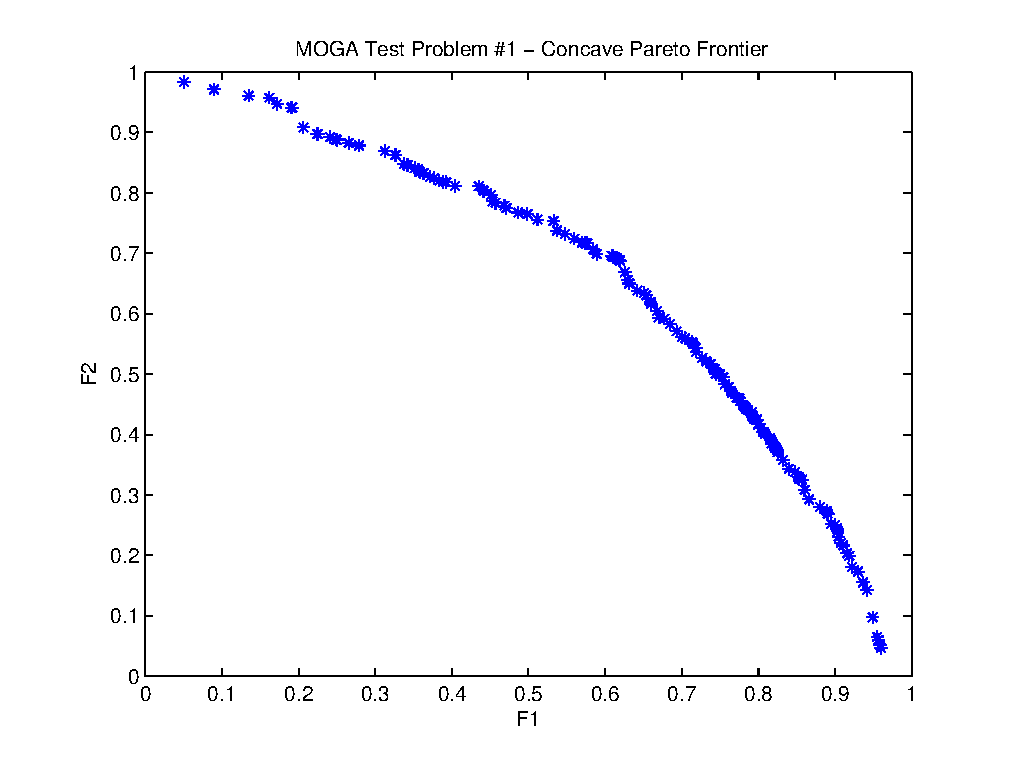
\includegraphics[scale=0.45]{../../images/mogatest1_pareto_front.eps}
    \caption{The Pareto Frontier of the Example Problem.}
    \label{fig:mogatest1_pareto_front}
\end{figure}

\section{Example 1 - A Minimal Implementation}\label{sec:example_1}
This section displays the minimal amount of code necessary to solve
this problem using JEGA.  It is not a "best-practice"
implementation.  To achieve the minimal implementation, this example
makes use of the core SimpleFunctorEvaluator and the associated
front end SimpleFunctorEvaluatorCreator.

As with any C++ program, we will need a main function.  As described
in Chapter~\ref{ch:configuration}, we will also need a problem
configuration object, an algorithm configuration object, an
evaluator and associated creator, and a parameter database.

\lstset{language=C++,
  commentstyle=\color{darkgreen}\sffamily\footnotesize,
}
\begin{lstlisting}[firstnumber=1,stepnumber=5,frame=single]{}
#include <cmath>
#include <memory>
#include <iostream>
#include <../FrontEnd/core/include/Driver.hpp>
#include <../FrontEnd/core/include/ProblemConfig.hpp>
#include <../FrontEnd/core/include/AlgorithmConfig.hpp>
#include <../Utilities/include/BasicParameterDatabaseImpl.hpp>
#include <../FrontEnd/core/include/SimpleFunctorEvaluatorCreator.hpp>

struct MyEvaluationFunctor :
    public JEGA::Algorithms::SimpleFunctorEvaluator::Functor
{
        virtual bool Evaluate(
            const JEGA::DoubleVector& X,
            JEGA::DoubleVector& F,
            JEGA::DoubleVector& G
            )
        {
            const std::size_t ndv = X.size();
            static const double sqrt3inv = 1.0/std::sqrt(3.0);

            F[0] = F[1] = 0.0;

            for(size_t dv=0; dv<ndv; ++dv) {
                F[0] += std::pow(X[dv] - (sqrt3inv), 2.0);
                F[1] += std::pow(X[dv] + (sqrt3inv), 2.0);
            }

            F[0] = 1.0 - std::exp(-F[0]);
            F[1] = 1.0 - std::exp(-F[1]);

            return true;
        }
};

int main(int argc, char* argv[])
{
    // All programs must initialize JEGA once and only once.
    JEGA::FrontEnd::Driver::InitializeJEGA(
        "JEGAGlobal.log", JEGA::Logging::ldebug(), 0
        );

    // Load up a problem config.
    JEGA::FrontEnd::ProblemConfig pConfig;
    pConfig.AddContinuumRealVariable("x1", -4.0, 4.0, 6);
    pConfig.AddContinuumRealVariable("x2", -4.0, 4.0, 6);
    pConfig.AddContinuumRealVariable("x3", -4.0, 4.0, 6);
    pConfig.AddNonlinearMinimizeObjective("F1");
    pConfig.AddNonlinearMinimizeObjective("F2");

    // Now load up an algorithm config for which we'll need a parameter
    // database and an evaluator creator.
    JEGA::Utilities::BasicParameterDatabaseImpl pdb;
    std::auto_ptr<MyEvaluationFunctor> ef(new MyEvaluationFunctor());
    JEGA::FrontEnd::SimpleFunctorEvaluatorCreator ec(ef.get());
    JEGA::FrontEnd::AlgorithmConfig aConfig(ec, pdb);

    // Start with algorithm level configuration.
    aConfig.SetAlgorithmType(JEGA::FrontEnd::AlgorithmConfig::MOGA);
    aConfig.SetDefaultLoggingLevel(JEGA::Logging::ldebug());
    aConfig.SetAlgorithmName("MOGA_1");
    aConfig.SetPrintPopEachGen(false);
    aConfig.SetOutputFilenamePattern("finaldata#.dat");

    // Now move on to operator configurations.
    aConfig.SetConvergerName("metric_tracker");
    pdb.AddIntegralParam("method.max_iterations", 2147483647);
    pdb.AddIntegralParam("method.max_function_evaluations", 3000);
    pdb.AddDoubleParam("method.jega.percent_change", 0.03);
    pdb.AddSizeTypeParam("method.jega.num_generations", 10);

    aConfig.SetCrosserName("multi_point_binary");
    pdb.AddDoubleParam("method.crossover_rate", 0.8);
    pdb.AddSizeTypeParam("method.jega.num_cross_points", 2);

    aConfig.SetNichePressureApplicatorName("distance");
    pdb.AddDoubleVectorParam(
        "method.jega.niche_vector", JEGA::DoubleVector(2, 0.05)
        );
    pdb.AddBooleanParam("method.jega.cache_niched_designs", true);

    aConfig.SetFitnessAssessorName("domination_count");

    aConfig.SetInitializerName("unique_random");
    pdb.AddIntegralParam("method.population_size", 50);

    aConfig.SetMainLoopName("duplicate_free");

    aConfig.SetMutatorName("replace_uniform");
    pdb.AddDoubleParam("method.mutation_rate", 0.1);

    aConfig.SetSelectorName("below_limit");
    pdb.AddDoubleParam("method.jega.fitness_limit", 4);
    pdb.AddDoubleParam("method.jega.shrinkage_percentage", 0.9);

    aConfig.SetPostProcessorName("null_postprocessor");

    // Now instantiate and use a Driver to get the
    // solutions to the problem.
    JEGA::FrontEnd::Driver app(pConfig);
    JEGA::Utilities::DesignOFSortSet res(
        app.ExecuteAlgorithm(aConfig)
        );

    // Do something with the solutions here.  We'll just print them
    // to the console for now.
    res.stream_out(std::cerr) << "\n\n";

    // YOU MUST FLUSH THE RETURNED SET OF SOLUTIONS
    // TO AVOID A MEMORY LEAK!!
    res.flush();
}
\end{lstlisting}
